\documentclass[11pt]{article}
\usepackage[margin=1in]{geometry}
\usepackage{amsmath}
\usepackage{booktabs}
\usepackage{float}
\usepackage{graphicx}

\title{ECON1750 Final Project: PCA Trading Strategies and Strategy Testing}
\date{}

\begin{document}
\maketitle

\section{Trading Strategies}

We build three strategies on top of the PCA factor model. The first, a \emph{contrarian factor-neutral Treynor--Black portfolio}, trades directly on the estimated alphas $\alpha_i$. The second, \emph{PCA pairs trading}, uses the principal component loadings to find pairs of economically similar stocks and trades the convergence of their prices. The third, \emph{residual snapback}, buys stocks whose recent returns fell far short of what the factor model predicted, betting that the overreaction reverses.

The data are daily returns for $N = 1{,}201$ stocks from January 2000 to December 2023. All three strategies are simulated out-of-sample: every estimate is recomputed on a trailing window as the simulation moves forward. Trading begins in January 2002 once 500 days of history are available (April 2002 for residual snapback, which also needs a residual history; see Section~\ref{sec:snapback}).

\subsection{Rolling factor model}

\begin{itemize}
    \item \textbf{Principal components.} Every 5 trading days, we run PCA on the correlation matrix of the previous 500 days of returns. Standardizing returns first prevents high-volatility stocks from dominating the components. We keep the top $K = 5$ eigenvectors $v_1, \dots, v_5$.
    \item \textbf{Factor returns.} Each eigenvector defines an eigenportfolio with return $f^k_t = \sum_i \frac{v_k[i]}{\bar\sigma_i} r_{i,t}$.
    \item \textbf{Alphas and betas.} Each day, for each stock, we regress the previous 250 days of returns on the five factor returns,
    \[
        r_{i,t} = \alpha_i + \sum_{k=1}^{K} \beta_{k,i} f^k_t + \epsilon_{i,t},
    \]
    which gives the alpha $\alpha_i$, the factor betas $\beta_{k,i}$, and the residual variance $\sigma^2(\epsilon_i)$.
\end{itemize}

\subsection{Strategy 1: Contrarian factor-neutral Treynor--Black}

\paragraph{Scores.} Under the Treynor--Black model, the optimal active weight on a stock is proportional to its alpha divided by its idiosyncratic variance: a large alpha on a very noisy stock deserves less weight than a moderate alpha on a stable one. We use the negative of this ratio,
\[
    s_i = -\frac{\alpha_i}{\sigma^2(\epsilon_i)}.
\]
The sign is flipped because, out of sample, stocks with high estimated alpha go on to \emph{underperform} (Table~\ref{tab:development}). Past alpha in this universe reverses: it reflects temporary mispricing or estimation noise, not persistent outperformance. Section~\ref{sec:holdout} confirms that this reversal is already present using only 2002--2017 data. To keep a few extreme stocks from dominating, we convert the scores to cross-sectional z-scores and cap them at $\pm 3$.

\paragraph{Factor neutrality.} We project the scores onto the space orthogonal to a vector of ones and the $K$ beta vectors, so the portfolio satisfies
\[
    \sum_i w_i = 0 \quad \text{(dollar neutral)}, \qquad \sum_i w_i \beta_{k,i} = 0 \quad \text{for } k = 1, \dots, K \quad \text{(factor neutral)}.
\]
Because the first principal component is essentially the market, this also makes the strategy approximately market neutral.

\paragraph{Scaling and trading.} Weights are scaled so gross exposure is $\sum_i |w_i| = 1$ (50\% long, 50\% short), and the portfolio is rebalanced daily.

\begin{table}[H]
\centering
\caption{Development of the strategy (out-of-sample, 2002--2023, 5bp fees unless stated).}
\label{tab:development}
\begin{tabular}{lrrrr}
\toprule
Strategy & Sharpe & Sharpe (no fees) & Return & Market beta \\
\midrule
Long top 20\% $\alpha$, short bottom 20\% & $-1.31$ & $-0.98$ & $-6.1\%$ & $-0.07$ \\
Contrarian 20\% sort & 0.66 & 0.98 & 3.1\% & 0.07 \\
Contrarian 20\% sort, factor-hedged & 0.72 & 1.12 & 2.9\% & 0.04 \\
Contrarian Treynor--Black, not hedged & 0.76 & 1.18 & 2.4\% & 0.07 \\
\textbf{Contrarian Treynor--Black, factor-hedged} & \textbf{0.85} & \textbf{1.31} & 2.5\% & 0.04 \\
\bottomrule
\end{tabular}
\end{table}

Each design choice helps. Reversing the sign turns a losing strategy into a profitable one. Weighting by $\alpha_i / \sigma^2(\epsilon_i)$ improves on equal weights. The factor hedge leaves the return almost unchanged (2.5\% vs.\ 2.4\%) but lowers volatility from 3.2\% to 2.9\% and market beta from 0.07 to 0.04: it removes unrewarded factor risk without sacrificing alpha. Market beta is measured against an equal-weighted average of all stocks in the universe.

\begin{figure}[H]
\centering
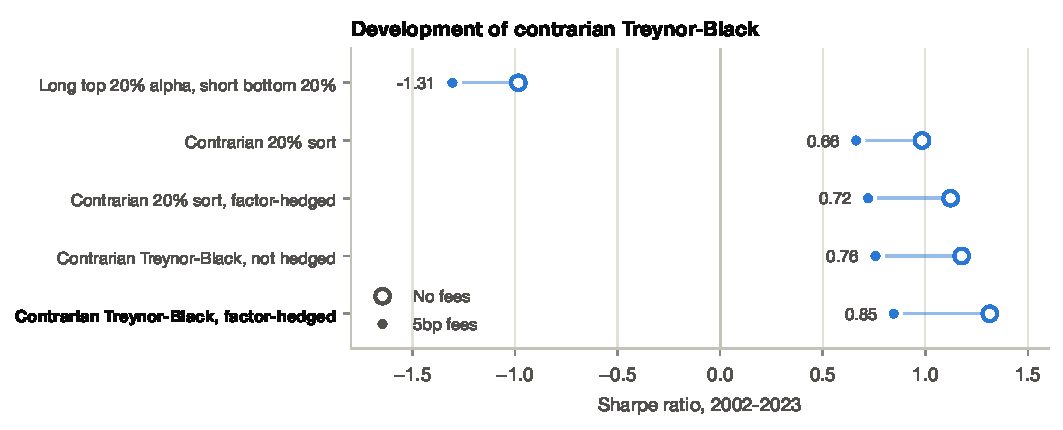
\includegraphics[width=0.85\textwidth]{figures/development_tb.pdf}
\caption{Development of the strategy (Table~\ref{tab:development}): Sharpe ratio of each step with 5bp fees (filled) and without fees (hollow).}
\label{fig:development-tb}
\end{figure}

\begin{figure}[H]
\centering
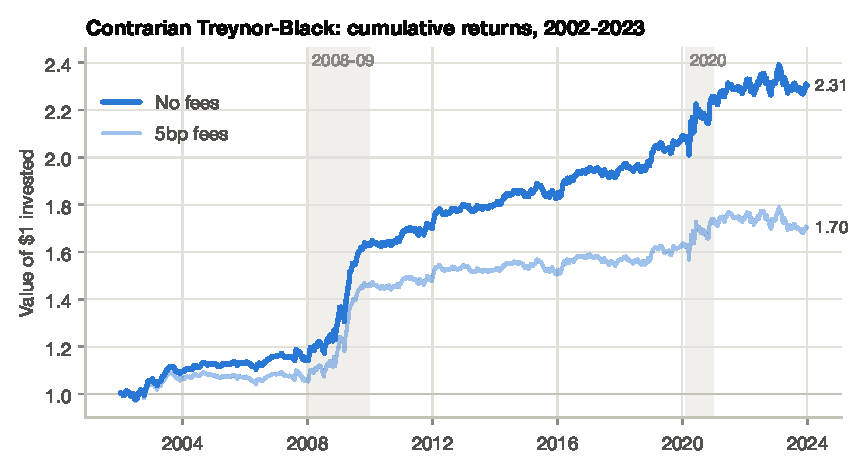
\includegraphics[width=\textwidth]{figures/cumulative_returns_tb.pdf}
\caption{Growth of \$1 invested in Contrarian Treynor--Black, with and without 5bp transaction costs. Shaded regions mark the 2008--09 financial crisis and the 2020 COVID crash.}
\label{fig:cumulative-tb}
\end{figure}

\begin{figure}[H]
\centering
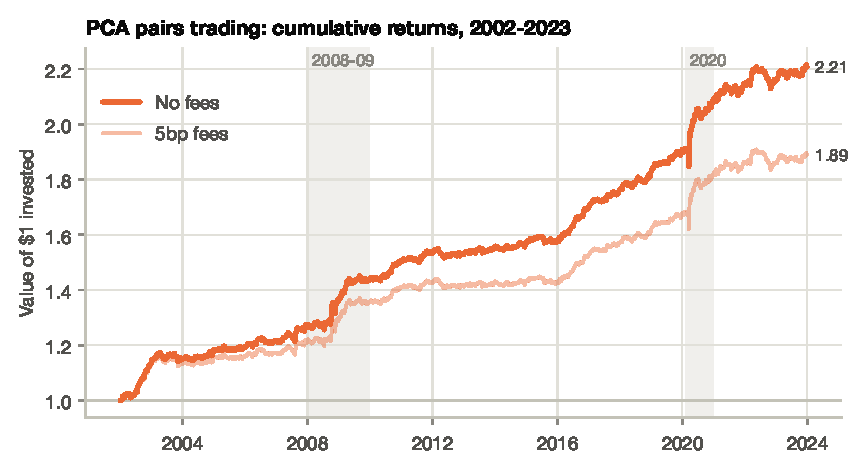
\includegraphics[width=\textwidth]{figures/cumulative_returns_pairs.pdf}
\caption{Growth of \$1 invested in PCA pairs trading, with and without 5bp transaction costs. Shaded regions mark the 2008--09 financial crisis and the 2020 COVID crash.}
\label{fig:cumulative-pairs}
\end{figure}

\subsection{Strategy 2: PCA pairs trading}

\paragraph{Pair selection.} Every 21 trading days, we describe each stock by its loadings on the $K$ principal components, $\ell_i = (v_1[i]\sqrt{\lambda_1}, \dots, v_K[i]\sqrt{\lambda_K})$. We then greedily match the closest stocks in this space, keeping the 50 best non-overlapping pairs. Because the two stocks in a pair have nearly identical factor exposure, the spread between them is approximately factor neutral and driven mostly by stock-specific news.

\paragraph{Trading rule.} For each pair $(i, j)$, we track the log price ratio $\log(P_i / P_j)$ over the previous 60 days and compute its z-score $z$. When $z < -2$ we buy $i$ and short $j$; when $z > 2$ we do the reverse. We close the position once $|z| < 0.5$. Each pair is allocated a fixed $1/50$ of capital, so idle pairs hold cash.

Even though no industry data is used, the selected pairs are economically sensible: utilities (WEC/DUK, ATO/NI), natural gas producers (EQT/CNX), tower REITs (AMT/SBAC) and apartment REITs (EQR/MAA). The principal components recover industry structure from returns alone.

\subsection{Strategy 3: Residual snapback}
\label{sec:snapback}

\paragraph{Idea.} The factor model splits each day's return into a part explained by the common factors and a stock-specific residual $\epsilon_{i,t}$. When a stock's residuals over the last few days are far more negative than usual, the stock has fallen much more than its factor exposures can explain. We treat this as an overreaction and buy the stock, expecting the gap to close. Treynor--Black trades on the \emph{level} of a stock's estimated alpha over the past year; snapback trades on a sharp, recent \emph{move} away from the model's prediction.

\paragraph{Lagged factor model.} Snapback uses its own version of the factor model. The PCA and the regression are fit on data through day $t-1$, and day $t$'s residual is then computed from those coefficients,
\[
    \epsilon_{i,t} = r_{i,t} - \alpha_i - \sum_{k=1}^{K} \beta_{k,i} f^k_t ,
\]
so the return being judged never enters the regression that judges it. The regression uses a 100-day window rather than Treynor--Black's 250 days. For Treynor--Black the alpha estimate \emph{is} the signal, so a long window reduces noise. For snapback the regression only provides a baseline for measuring surprises, and a shorter window lets that baseline follow recent changes in each stock's factor exposures, at the cost of noisier coefficient estimates.

\paragraph{Score.} A residual of $-5\%$ is extreme for a stable utility but routine for a volatile biotech, so we measure each residual against the stock's typical residual size. Let $\hat\sigma_{i,t}$ be the sample standard deviation of stock $i$'s residuals over the 60 days before the last three,
\[
    \hat\sigma_{i,t} = \sqrt{\frac{1}{59} \sum_{k=3}^{62} \left(\epsilon_{i,t-k} - \bar\epsilon_{i,t}\right)^2},
    \qquad
    \bar\epsilon_{i,t} = \frac{1}{60} \sum_{k=3}^{62} \epsilon_{i,t-k} .
\]
The score is the sum of the last three residuals in units of their expected spread,
\[
    s_{i,t} = \frac{\epsilon_{i,t-2} + \epsilon_{i,t-1} + \epsilon_{i,t}}{\sqrt{3}\, \hat\sigma_{i,t}} .
\]
The numerator is how far the stock has fallen short of (if negative) or run ahead of (if positive) the factor model over three days. If residuals have mean zero and are uncorrelated from day to day, the sum of three has variance $3\sigma_i^2$, so dividing by $\sqrt{3}\,\hat\sigma_{i,t}$ puts the score in standard-deviation units. Under these assumptions $s_{i,t}$ is roughly a standard normal draw, and $s_{i,t} \le -2$ marks an unusually large shortfall.

\paragraph{Checking the assumptions.} Both assumptions can be tested on the residuals themselves (Table~\ref{tab:residuals}). If the lagged model were biased, a negative residual sum could reflect the model's own error rather than a genuine shortfall. It is not biased: the mean residual across all stocks and days is $-0.003$bp per day ($t = -0.02$). The average across stocks of each stock's 60-day mean residual stays within a few basis points of zero throughout 2002--2023, including 2008--09 and 2020 (Figure~\ref{fig:residual-means}). Individual stocks' 60-day means spread about $\pm 25$bp per day (10th to 90th percentile), no wider than sampling noise alone would produce: with a typical daily residual volatility of 1.8\%, a 60-day mean has a standard error of about 23bp. One might expect the second assumption to fail in the other direction: if overreaction persists for several days, residuals would be positively correlated and $\sqrt{3}$ would understate the spread of their sum. In fact residuals are slightly \emph{negatively} correlated (median lag-1 autocorrelation $-0.03$), so a three-day sum varies about 5\% less than $\sqrt{3}$ assumes. The reversal the strategy bets on already begins within the three days. The $\sqrt{3}$ scaling is therefore close to right. Because it applies to every stock alike, a small error in it would mainly change how many stocks pass the $-2$ cutoff, not which stocks rank lowest. Across all stocks and days the scores have a standard deviation of 1.08, slightly above 1, because $\hat\sigma_{i,t}$ is estimated from only 60 days and residuals have fat tails.

\begin{table}[H]
\centering
\caption{Residual diagnostics: lagged factor model, every stock and trading day, April 2002--2023.}
\label{tab:residuals}
\begin{tabular}{lr}
\toprule
Measure & Value \\
\midrule
Mean residual (bp per day) & $-0.003$ \\
Newey--West $t$-statistic of the daily cross-sectional mean & $-0.02$ \\
Median daily residual volatility & 1.8\% \\
60-day mean residual, 10th / 90th percentile across stocks (bp per day) & $-25$ / 24 \\
Median autocorrelation of residuals, lag 1 / lag 2 & $-0.034$ / $-0.009$ \\
Median variance of 3-day sum / (3 $\times$ daily variance) & 0.95 \\
Standard deviation of the snapback score & 1.08 \\
\bottomrule
\end{tabular}
\end{table}

\begin{figure}[H]
\centering
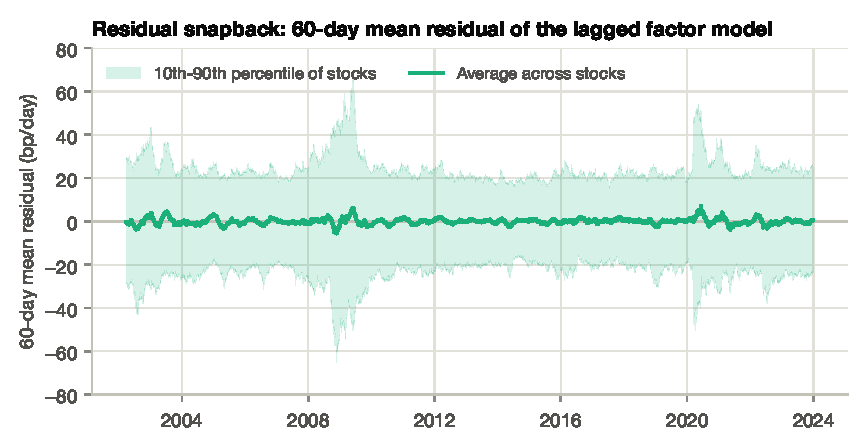
\includegraphics[width=\textwidth]{figures/residual_means.pdf}
\caption{Residual diagnostics (Table~\ref{tab:residuals}): each stock's trailing 60-day mean residual from the lagged factor model. The line is the average across stocks, the band the 10th to 90th percentile.}
\label{fig:residual-means}
\end{figure}

\paragraph{Long-only version (default).} On the last trading day of each week we buy up to 20 stocks with the lowest scores, among those with $s_{i,t} \le -2$, in equal weights, and hold them until the next rebalance. If no stock qualifies, the portfolio holds cash. This default version is \emph{long only}, so it also carries the market.

\paragraph{Fully hedged version.} Even if the signal picks stocks that will beat the market, the long-only portfolio carries their factor exposures: an equal-weighted basket of stocks that have just fallen can load heavily on the market or on a sector-like component. The fully hedged version removes this exposure by trading the signal on both sides. On each rebalance date it takes up to 40 stocks with the lowest scores at or below $-2$ as long candidates and up to 40 stocks with the highest scores at or above $+2$ as short candidates, betting that stocks that ran unusually far ahead of the model will fall back. The starting weights $w^{(0)}_t$ put half the capital equally into the longs and half equally into the shorts: $w^{(0)}_{i,t} = 0.5 / n_L$ for each of the $n_L$ long candidates and $-0.5 / n_S$ for each of the $n_S$ short candidates. Let $B_t$ be the $K \times (n_L + n_S)$ matrix of the candidates' estimated betas, so $B_t w_t$ is the portfolio's factor exposure. We choose the weights closest to the starting weights that are factor neutral, have gross exposure 1 and keep the direction of each trade:
\[
\begin{aligned}
\min_{w_t} \quad & \tfrac{1}{2} \lVert w_t - w^{(0)}_t \rVert_2^2 \\
\text{subject to} \quad & B_t w_t = 0, \qquad \textstyle\sum_i |w_{i,t}| = 1, \\
& w_{i,t} \ge 0 \text{ for long candidates}, \qquad w_{i,t} \le 0 \text{ for short candidates}.
\end{aligned}
\]
Because each weight's sign is fixed, the gross-exposure constraint is linear, so this is a convex quadratic program; we solve it numerically (SLSQP). If either side has no candidates, or no weights satisfy the constraints, the hedged portfolio holds cash. The weights are not forced to be dollar neutral, but since the first factor is essentially the market, the portfolio is close to market neutral. An earlier version hedged only the long picks, projecting their equal weights onto the null space of their betas, which could short some of the 20 picks regardless of their scores. We keep it as a comparison row in Table~\ref{tab:snapback-variants}.

\paragraph{Fixed-weight hybrids.} The long-only version has the higher return; the hedged version has less risk. The hybrids construct both portfolios exactly as above and combine their weights,
\[
    w_t^{\text{hybrid}} = \lambda\, w_t^{\text{long only}} + (1 - \lambda)\, w_t^{\text{hedged}},
\]
for $\lambda = 0.7$, 0.5 and 0.3, to test whether a blend keeps some of the long-only upside while reducing exposure to common factor moves.

\paragraph{Volatility-weighted hybrid (dynamic).} A fixed $\lambda$ treats calm and turbulent markets alike, although factor risk matters most when markets are volatile. The dynamic version hedges more when volatility is high. Each day we compute the return of the equal-weighted universe and its sample standard deviation over the trailing 30 trading days. On each rebalance date we compare the current reading with all $n_t$ earlier readings and count the $k_t$ that are lower, with ties counting $\tfrac12$. The raw percentile $k_t / n_t$ is unstable when there are few earlier readings: the very first reading is both the highest and the lowest seen so far. We therefore add 126 pseudo-readings on each side (Laplace smoothing). The hedged weight is
\[
    \tilde p_t = \frac{k_t + 126}{n_t + 252}, \qquad
    w_t^{\text{dynamic}} = (1 - \tilde p_t)\, w_t^{\text{long only}} + \tilde p_t\, w_t^{\text{hedged}} .
\]
With no earlier readings the mix starts at 50/50, and the starting mix gets weight $252 / (n_t + 252)$, which shrinks as readings accumulate. For example, with 252 earlier readings a raw percentile of 90\% becomes a hedged weight of 70\%. When trading begins in 2002 about 470 readings are available, so the smoothing pulls the raw percentile about a third of the way towards 50\%; by 2023 the pull is about 4\% (Figure~\ref{fig:hedge-allocation}). An earlier version used the raw percentile and stayed fully long-only until 252 readings had accumulated; we keep it as a comparison row.

\begin{figure}[H]
\centering
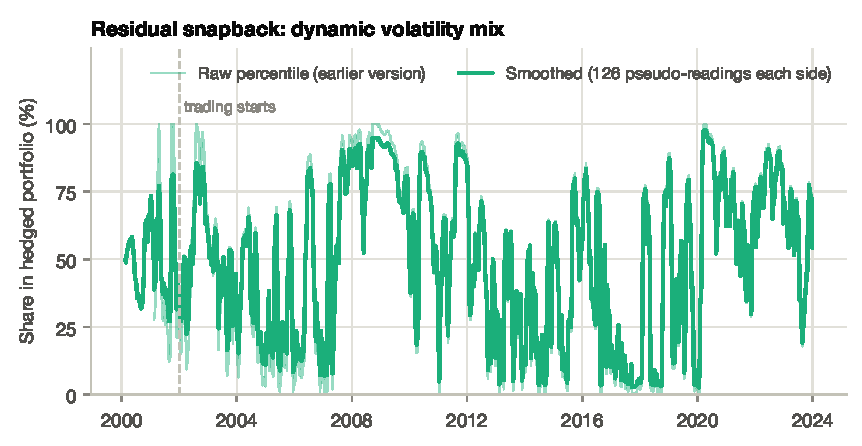
\includegraphics[width=\textwidth]{figures/hedge_allocation.pdf}
\caption{Dynamic volatility mix: share of the portfolio in the fully hedged book at each weekly rebalance, using the smoothed percentile $\tilde p_t$ (dark) and the raw percentile of the earlier version (light).}
\label{fig:hedge-allocation}
\end{figure}

\paragraph{Cumulative residual score.} The snapback score only looks at the last three days. A stock that drifts below the factor model for weeks but then trades in line with it for three days has a snapback score near zero, even though its cumulative shortfall may be large. The cumulative score captures such drifts. We add each day's residual to a running total and compare today's level with its previous 60 levels:
\[
    X_{i,t} = X_{i,t-1} + \epsilon_{i,t}, \qquad
    z_{i,t} = \frac{X_{i,t} - \overline{X}^{(60)}_{i,t}}{s^{(60)}_{i,t}},
\]
where $\overline{X}^{(60)}_{i,t}$ and $s^{(60)}_{i,t}$ are the mean and sample standard deviation of $X_{i,t-60}, \dots, X_{i,t-1}$. The 60 days provide the reference level and scale, while the running total itself carries forward from day to day. A negative score means the running total is unusually far below its recent levels, and the hypothesis is again that unusually low levels rise and unusually high levels fall. The two scores are related but distinct: across all stocks and days their correlation is 0.47. We trade the cumulative score in two ways. First, with exactly the snapback rules above (weekly, long only or the 40/40 long-short book, cutoff $\pm 2$), using the same lagged factor model, so the only change is the score. Second, as a \emph{daily rank book}, the version developed on our group's residual-reversion branch: every day it buys the 20\% of stocks with the lowest scores and shorts the 20\% with the highest, with at most 2\% in any stock, then shrinks positions until the book is both dollar and factor neutral. This version uses an unlagged regression refit every five days, as on that branch.

\begin{table}[H]
\centering
\caption{Residual snapback variants (out-of-sample, April 2002--2023).}
\label{tab:snapback-variants}
\begin{tabular}{lrrrrrr}
\toprule
Variant & Sharpe & Sharpe (no fees) & Return & Volatility & Market beta & Max drawdown \\
\midrule
Equal-weight benchmark & 0.82 & 0.83 & 14.7\% & 18.8\% & 1.00 & $-53.0\%$ \\
\textbf{Long only (default)} & \textbf{0.82} & \textbf{1.03} & 19.1\% & 25.2\% & 1.08 & $-58.5\%$ \\
Stricter cutoff ($s_i \le -2.5$) & 0.67 & 0.86 & 15.3\% & 26.5\% & 1.08 & $-74.8\%$ \\
Hybrid, 70\% long only & 0.87 & 1.14 & 15.7\% & 18.8\% & 0.77 & $-45.0\%$ \\
Hybrid, 50\% long only & 0.91 & 1.26 & 13.1\% & 14.8\% & 0.57 & $-36.1\%$ \\
Hybrid, 30\% long only & 0.94 & 1.39 & 10.4\% & 11.3\% & 0.36 & $-30.3\%$ \\
Dynamic volatility mix & 0.96 & 1.39 & 11.3\% & 11.9\% & 0.31 & $-27.8\%$ \\
\textbf{Fully hedged (long-short)} & \textbf{0.76} & \textbf{1.38} & 6.1\% & 8.2\% & 0.06 & $-21.5\%$ \\
\midrule
\multicolumn{7}{l}{\emph{Earlier versions, for comparison}} \\
Projection hedge of the long picks & 0.83 & 1.23 & 10.2\% & 12.7\% & 0.12 & $-28.7\%$ \\
Dynamic mix, unsmoothed, projection hedge & 1.00 & 1.33 & 13.4\% & 13.5\% & 0.33 & $-32.8\%$ \\
\midrule
\multicolumn{7}{l}{\emph{Cumulative residual score}} \\
Long only (snapback rules) & 1.18 & 1.36 & 28.9\% & 23.9\% & 1.08 & $-53.2\%$ \\
Long-short (snapback rules) & 1.76 & 2.36 & 12.6\% & 6.9\% & 0.07 & $-10.4\%$ \\
Daily rank book & 3.01 & 4.41 & 9.5\% & 3.0\% & 0.05 & $-8.3\%$ \\
\bottomrule
\end{tabular}
\\[4pt]
\small 5bp fees unless stated. The benchmark holds every stock in equal weights, rebalanced weekly. Market beta is measured against the equal-weighted universe, as in Table~\ref{tab:development}.
\end{table}

The long-only default earns 19.1\% a year, but its Sharpe ratio after fees (0.82) only matches the equal-weight benchmark: most of its return and nearly all of its risk come from the market (beta 1.08). Regressing its daily returns on the market leaves an alpha of 3.6\% a year with 14.0\% residual volatility, an information ratio of 0.26. Hedging removes the market: the fully hedged long-short version has beta 0.06 and a market-adjusted alpha of 5.3\% a year with 8.2\% residual volatility (information ratio 0.65, close to Treynor--Black's 0.64 and below pairs trading's 1.05). Before fees its Sharpe ratio (1.38) is well above the long-only version's (1.03), but it trades as much as the long-only version on a smaller return, so after fees it falls to 0.76. Compared with the earlier projection hedge, the long-short book has lower risk (8.2\% vs.\ 12.7\% volatility, $-21.5\%$ vs.\ $-28.7\%$ drawdown) and a higher Sharpe ratio before fees (1.38 vs.\ 1.23), but a lower one after fees (0.76 vs.\ 0.83) and less alpha (5.3\% vs.\ 8.6\%). The hybrids and the dynamic mix have the highest Sharpe ratios after fees (0.87--0.96) because the long-only and hedged returns are imperfectly correlated. The mixes were chosen with the full sample in view; Section~\ref{sec:holdout} checks them out-of-sample. Because the long-only default is what the strategy was designed as, and the fully hedged version is the one comparable to the two market-neutral strategies, we test both throughout.

\begin{figure}[H]
\centering
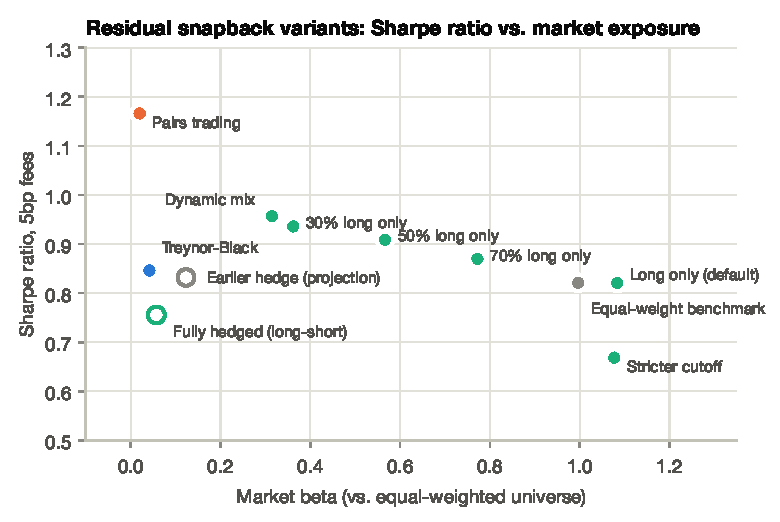
\includegraphics[width=0.75\textwidth]{figures/snapback_variants.pdf}
\caption{Residual snapback variants (Table~\ref{tab:snapback-variants}): Sharpe ratio with 5bp fees against market beta. Hollow markers are long-short books. The earlier projection hedge (gray) and the two market-neutral strategies are shown for reference. The daily rank book (Sharpe 3.01) is off scale.}
\label{fig:snapback-variants}
\end{figure}

Replacing the snapback score with the cumulative score improves both versions substantially, with nothing else changed: the long-only Sharpe ratio after fees rises from 0.82 to 1.18 and the long-short one from 0.76 to 1.76, above pairs trading's 1.17. The cumulative score also trades less (about 80--87 times a year rather than 100), so the long-short version breaks even at 20bp rather than 11bp. Both improvements hold in the 2018--2023 holdout (Table~\ref{tab:delay}). The daily rank book reaches a Sharpe ratio of 3.01 after fees (2.70 from 2004, reproducing the residual-reversion branch's result exactly).

Results this strong call for a check of how they would be executed. All our backtests trade at the closing price of the day the signal is computed. If part of a stock's residual on that day is noise in the closing price, such as a trade at the bid or the ask, the price partly reverts the next day. Trading at that same close then captures a reversal that could not be traded in practice. Table~\ref{tab:delay} repeats each version with every trade executed one day late. The daily rank book collapses from 3.01 to 0.25: almost all of its profit comes from the first day after the signal. The original snapback long-short book falls from 0.76 to 0.16. The weekly cumulative versions are the most robust, keeping a Sharpe ratio of 0.97 (long only) and 1.07 (long-short) when executed a day late. Their edge comes from a reversal that builds over weeks, not from the next day's bounce.

\begin{table}[H]
\centering
\caption{Execution delay: Sharpe ratios (5bp fees) when trading at the signal's close and one day later.}
\label{tab:delay}
\begin{tabular}{lrrrrr}
\toprule
& \multicolumn{2}{c}{Full period} & \multicolumn{2}{c}{At the signal's close} & \\
\cmidrule(lr){2-3} \cmidrule(lr){4-5}
Version & At close & One day late & 2002--2017 & 2018--2023 & Break-even fee \\
\midrule
Snapback score, long only & 0.82 & 0.65 & 0.91 & 0.62 & 25bp \\
Snapback score, long-short & 0.76 & 0.16 & 0.85 & 0.59 & 11bp \\
Cumulative score, long only & 1.18 & 0.97 & 1.27 & 0.97 & 37bp \\
Cumulative score, long-short & 1.76 & 1.07 & 2.03 & 1.26 & 20bp \\
Daily rank book & 3.01 & 0.25 & 3.93 & 1.43 & 16bp \\
\bottomrule
\end{tabular}
\\[4pt]
\small Each version from its first trade (April 2002). The selection and holdout columns therefore differ slightly from Table~\ref{tab:holdout}, which uses a common period from March 2004.
\end{table}

\begin{figure}[H]
\centering
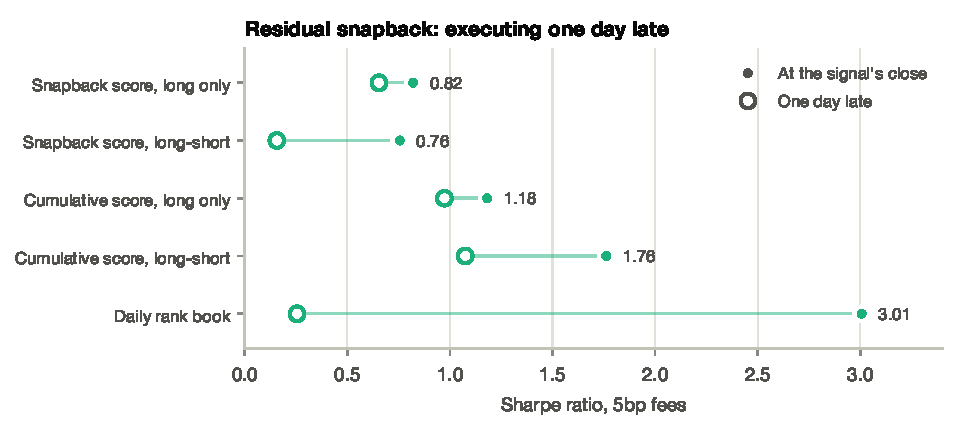
\includegraphics[width=0.85\textwidth]{figures/execution_delay.pdf}
\caption{Execution delay (Table~\ref{tab:delay}): Sharpe ratio with 5bp fees when trading at the signal's close (filled) and one day later (hollow).}
\label{fig:execution-delay}
\end{figure}

\begin{figure}[H]
\centering
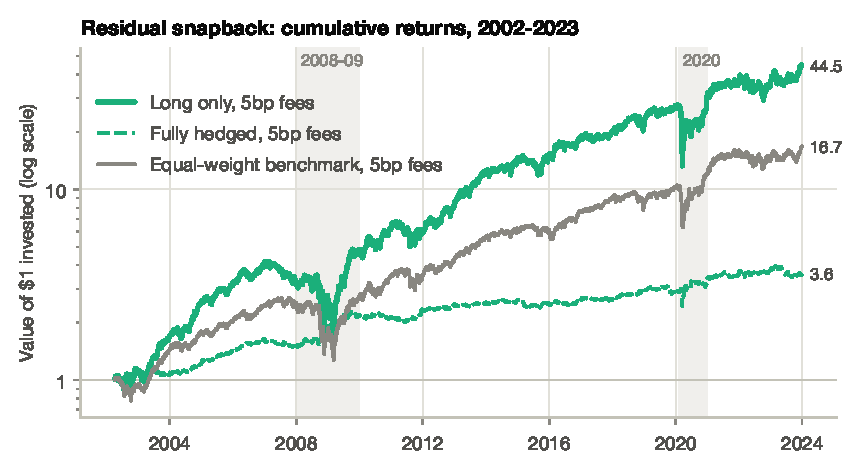
\includegraphics[width=\textwidth]{figures/cumulative_returns_snap.pdf}
\caption{Growth of \$1 invested in residual snapback (long only and fully hedged) and the equal-weight benchmark, with 5bp transaction costs, on a log scale. Shaded regions mark the 2008--09 financial crisis and the 2020 COVID crash.}
\label{fig:cumulative-snap}
\end{figure}

\subsection{Backtest design}

\paragraph{Timing and look-ahead bias.} Weights chosen at the close of day $t$ use only returns up to and including day $t$, and they earn the returns of day $t+1$: $r_{\text{port},t+1} = \sum_i w_{i,t} r_{i,t+1}$. We verified this directly: re-running the backtest on data truncated at December 2011 leaves every earlier position unchanged, up to floating-point rounding of order $10^{-13}$. Residual snapback follows the same convention and additionally fits its factor model only through day $t-1$. Between weekly rebalances its positions drift with prices and are not traded.

\paragraph{Transaction costs.} The assignment defines returns without costs, so we report results both without fees and with a cost of 5 basis points per dollar traded.

\paragraph{Survivorship bias.} Every stock in the sample trades continuously from 2000 to 2023, so the universe consists of firms that survived the full period. Firms that failed or were acquired are missing. This likely flatters all three strategies, since buying a stock after a fall never ends in a delisting in this sample. Residual snapback is the most exposed, because buying stocks right after unusually large drops is its entire signal. This is a limitation of the data, not of the strategy code.

\section{Strategy Testing}

We test all three strategies along six dimensions, reporting residual snapback in both its long-only and fully hedged forms. Unless stated otherwise, all results are out-of-sample, from January 2002 (April 2002 for snapback) to December 2023.

\subsection{Regime robustness}

\begin{table}[H]
\centering
\caption{Annual returns and Sharpe ratios.}
\label{tab:yearly}
\begin{tabular}{lrrrrrr}
\toprule
& \multicolumn{3}{c}{Contrarian Treynor--Black} & \multicolumn{3}{c}{PCA pairs trading} \\
\cmidrule(lr){2-4} \cmidrule(lr){5-7}
Year & Return & Return (5bp) & Sharpe & Return & Return (5bp) & Sharpe \\
\midrule
2002 & 5.6\% & 4.2\% & 1.93 & 13.8\% & 13.0\% & 3.52 \\
2003 & 3.6\% & 2.2\% & 1.64 & 0.9\% & 0.1\% & 0.33 \\
2004 & 2.6\% & 1.2\% & 1.51 & 2.6\% & 1.9\% & 1.02 \\
2005 & 0.7\% & $-0.7\%$ & 0.40 & 1.4\% & 0.7\% & 0.69 \\
2006 & 2.4\% & 1.1\% & 1.29 & 1.6\% & 0.8\% & 0.85 \\
2007 & $-1.1\%$ & $-2.4\%$ & $-0.38$ & 4.8\% & 4.0\% & 1.77 \\
2008 & 15.6\% & 13.7\% & 3.00 & 7.2\% & 6.2\% & 1.53 \\
2009 & 23.4\% & 21.5\% & 4.83 & 5.5\% & 4.8\% & 2.02 \\
2010 & 2.2\% & 0.8\% & 1.14 & 4.8\% & 4.1\% & 2.49 \\
2011 & 2.3\% & 0.8\% & 0.90 & 2.1\% & 1.3\% & 1.12 \\
2012 & 5.3\% & 3.9\% & 2.58 & $-0.6\%$ & $-1.2\%$ & $-0.42$ \\
2013 & 0.2\% & $-1.1\%$ & 0.14 & 1.8\% & 1.1\% & 0.94 \\
2014 & 2.7\% & 1.3\% & 1.62 & 1.1\% & 0.4\% & 0.79 \\
2015 & $-0.3\%$ & $-1.6\%$ & $-0.14$ & 0.1\% & $-0.6\%$ & 0.07 \\
2016 & 5.5\% & 4.1\% & 2.50 & 7.8\% & 7.0\% & 3.80 \\
2017 & 0.3\% & $-0.9\%$ & 0.14 & 3.9\% & 3.2\% & 2.28 \\
2018 & 1.7\% & 0.4\% & 0.70 & 3.6\% & 2.8\% & 2.06 \\
2019 & 5.1\% & 3.7\% & 2.46 & 4.5\% & 3.9\% & 2.71 \\
2020 & 8.1\% & 6.5\% & 1.26 & 9.5\% & 8.6\% & 1.91 \\
2021 & 1.6\% & 0.1\% & 0.61 & 2.7\% & 2.1\% & 1.14 \\
2022 & 1.6\% & 0.2\% & 0.44 & 0.7\% & $-0.1\%$ & 0.32 \\
2023 & $-0.8\%$ & $-2.1\%$ & $-0.22$ & 2.2\% & 1.6\% & 1.05 \\
\bottomrule
\end{tabular}
\\[4pt]
\small Returns and Sharpe ratios are without fees unless marked 5bp.
\end{table}

\begin{table}[H]
\centering
\caption{Annual returns and Sharpe ratios: residual snapback.}
\label{tab:yearly-snap}
\begin{tabular}{lrrrrrr}
\toprule
& \multicolumn{3}{c}{Long only} & \multicolumn{3}{c}{Fully hedged} \\
\cmidrule(lr){2-4} \cmidrule(lr){5-7}
Year & Return & Return (5bp) & Sharpe & Return & Return (5bp) & Sharpe \\
\midrule
2002 & 14.1\% & 9.9\% & 0.77 & 13.8\% & 9.7\% & 1.97 \\
2003 & 64.3\% & 56.1\% & 3.28 & 5.2\% & 0.0\% & 0.71 \\
2004 & 59.0\% & 50.9\% & 2.79 & 17.6\% & 11.7\% & 2.50 \\
2005 & 27.1\% & 20.7\% & 1.90 & 21.6\% & 15.5\% & 3.78 \\
2006 & 36.2\% & 29.4\% & 2.26 & 19.7\% & 13.7\% & 3.49 \\
2007 & $-14.9\%$ & $-19.1\%$ & $-0.79$ & $-1.4\%$ & $-6.3\%$ & $-0.18$ \\
2008 & $-20.7\%$ & $-24.6\%$ & $-0.18$ & 25.7\% & 19.6\% & 1.67 \\
2009 & 104.7\% & 94.3\% & 1.87 & 27.1\% & 20.9\% & 1.98 \\
2010 & 35.7\% & 28.9\% & 1.58 & 2.7\% & $-2.5\%$ & 0.44 \\
2011 & 1.5\% & $-3.5\%$ & 0.19 & 15.6\% & 9.8\% & 2.30 \\
2012 & 45.8\% & 38.5\% & 2.48 & 12.8\% & 7.2\% & 1.91 \\
2013 & 58.9\% & 51.0\% & 3.26 & 7.5\% & 2.2\% & 1.63 \\
2014 & 20.4\% & 14.3\% & 1.36 & 7.8\% & 2.4\% & 1.56 \\
2015 & 11.8\% & 6.1\% & 0.68 & 1.4\% & $-3.8\%$ & 0.26 \\
2016 & 28.5\% & 22.1\% & 1.60 & 8.9\% & 3.4\% & 1.44 \\
2017 & 13.8\% & 8.1\% & 1.16 & 5.9\% & 0.6\% & 1.05 \\
2018 & 13.2\% & 7.5\% & 0.85 & 17.7\% & 11.9\% & 3.20 \\
2019 & 34.3\% & 27.6\% & 2.06 & 4.3\% & $-0.9\%$ & 0.69 \\
2020 & 20.5\% & 14.5\% & 0.62 & 23.4\% & 18.0\% & 1.26 \\
2021 & 24.1\% & 17.9\% & 1.35 & 10.2\% & 4.7\% & 1.37 \\
2022 & 1.2\% & $-3.9\%$ & 0.18 & 9.4\% & 4.0\% & 1.10 \\
2023 & 31.9\% & 25.3\% & 1.49 & 1.3\% & $-3.7\%$ & 0.21 \\
\bottomrule
\end{tabular}
\\[4pt]
\small Returns and Sharpe ratios are without fees unless marked 5bp. 2002 starts in April.
\end{table}

\begin{table}[H]
\centering
\caption{Concentration and stability of returns.}
\label{tab:regime}
\resizebox{\textwidth}{!}{%
\begin{tabular}{lcccc}
\toprule
& & & \multicolumn{2}{c}{Residual snapback} \\
\cmidrule(lr){4-5}
Measure & Treynor--Black & Pairs trading & Long only & Fully hedged \\
\midrule
Years positive (no fees / 5bp) & 19 / 16 of 22 & 21 / 19 of 22 & 20 / 18 of 22 & 21 / 16 of 22 \\
Share of total profit from best year & 25\% (2009) & 16\% (2002) & 15\% (2009) & 10\% (2009) \\
Share of total profit from best two years & 43\% (2008--09) & 28\% (2002, 2020) & 25\% (2003, 2009) & 20\% (2008, 2009) \\
Sharpe, all years (no fees / 5bp) & 1.31 / 0.85 & 1.45 / 1.17 & 1.03 / 0.82 & 1.38 / 0.76 \\
Sharpe excluding best two years (no fees / 5bp) & 0.91 / 0.41 & 1.28 / 0.97 & 0.90 / 0.68 & 1.34 / 0.65 \\
Sharpe 2002--2012 / 2013--2023 (5bp) & 1.41 / 0.32 & 1.18 / 1.16 & 0.86 / 0.78 & 1.06 / 0.45 \\
Maximum drawdown (no fees / 5bp) & $-5.2\%$ / $-6.1\%$ & $-3.6\%$ / $-3.9\%$ & $-54.6\%$ / $-58.5\%$ & $-19.6\%$ / $-21.5\%$ \\
\bottomrule
\end{tabular}}
\end{table}

No single year carries any of the strategies, but they differ markedly (Figures~\ref{fig:cumulative-tb}--\ref{fig:annual-snap}). Treynor--Black earns its best returns in crises: in 2008 it gained 15.6\% while the market fell 27\%, followed by 23.4\% in 2009 and 8.1\% in 2020. These are periods of panic selling and overreaction, when betting on reversal should pay. However, 2008--09 account for 43\% of its total profit, and its Sharpe ratio after fees fell from 1.41 in 2002--2012 to 0.32 in 2013--2023. Pairs trading is far more stable: profitable in 21 of 22 years, no more than 28\% of profit from any two years, and an essentially identical Sharpe ratio in both halves of the sample.

Residual snapback has the least concentrated profits of the three: its best two years supply only about a quarter of the total. But it behaves very differently in crises. Long-only snapback lost 19.1\% in 2007 while the market rose 2\%, and 24.6\% in 2008, then gained 94\% in 2009. Buying the stocks that have just fallen hardest means catching falling knives in a sustained sell-off, and the long-only version carries the full market drawdown on top ($-58.5\%$ peak to trough, versus $-53\%$ for the benchmark). The fully hedged version behaves more like Treynor--Black: 2008 (25.7\%) and 2009 (27.1\%) are its two best years, and it cuts the maximum drawdown to $-21.5\%$. But its edge has faded: its Sharpe ratio after fees fell from 1.06 in 2002--2012 to 0.45 in 2013--2023, the second-largest decline after Treynor--Black's. Since 2013 it has lost money after fees in 2015, 2019 and 2023 and earned less than 2.5\% in 2013, 2014 and 2017.

\begin{figure}[H]
\centering
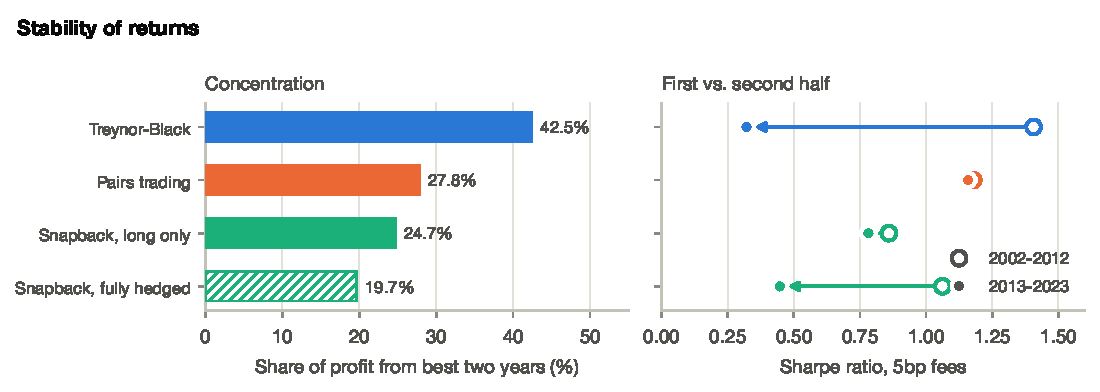
\includegraphics[width=\textwidth]{figures/regime_stability.pdf}
\caption{Concentration and stability of returns (Table~\ref{tab:regime}). Left: share of total profit (no fees) earned in each strategy's best two years. Right: Sharpe ratio with 5bp fees in 2002--2012 (hollow) and 2013--2023 (filled).}
\label{fig:regime-stability}
\end{figure}

\begin{figure}[H]
\centering
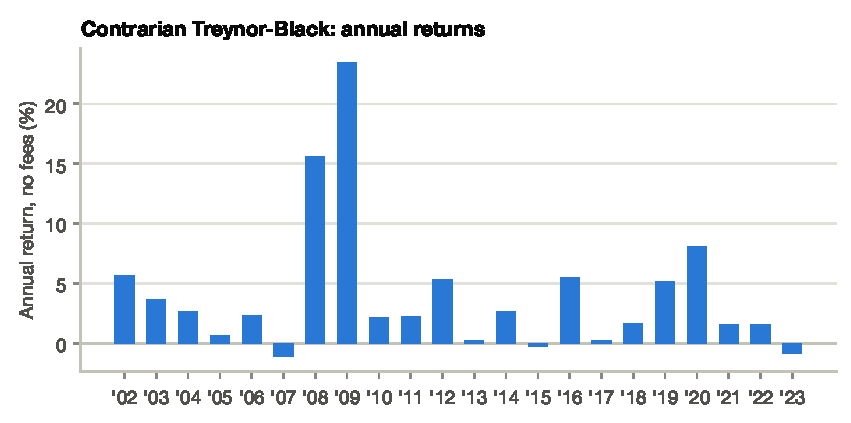
\includegraphics[width=\textwidth]{figures/annual_returns_tb.pdf}
\caption{Annual returns of Contrarian Treynor--Black (no fees).}
\label{fig:annual-tb}
\end{figure}

\begin{figure}[H]
\centering
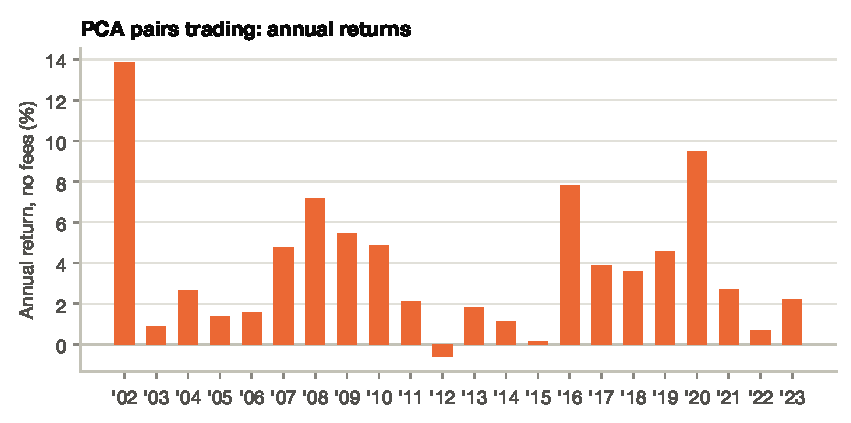
\includegraphics[width=\textwidth]{figures/annual_returns_pairs.pdf}
\caption{Annual returns of PCA pairs trading (no fees).}
\label{fig:annual-pairs}
\end{figure}

\begin{figure}[H]
\centering
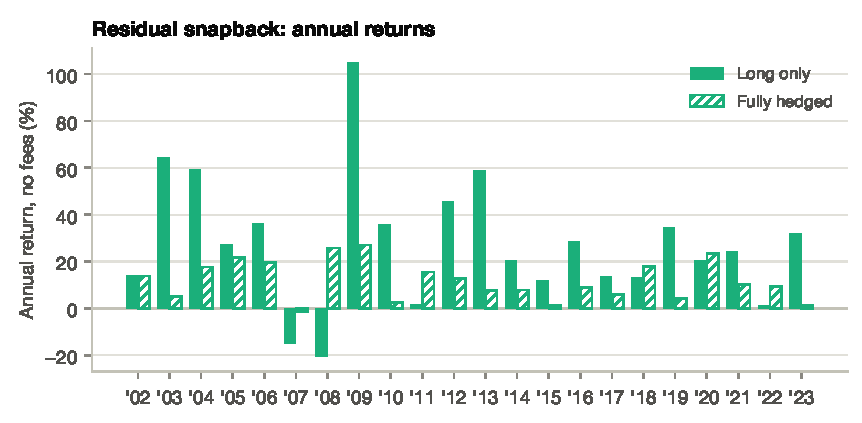
\includegraphics[width=\textwidth]{figures/annual_returns_snap.pdf}
\caption{Annual returns of residual snapback, long only (solid) and fully hedged (hatched), no fees. 2002 starts in April.}
\label{fig:annual-snap}
\end{figure}

\subsection{Parameter sensitivity}

We vary one parameter at a time around the defaults. Because a 1000-day PCA window needs four years of history, all variants are compared over a common period: December 2003 onward for Treynor--Black and pairs trading, and March 2004 onward for residual snapback, whose lagged model and residual history need a few more months. The selection and holdout columns split this period into a selection period (through 2017) and a holdout period (2018--2023); see Section~\ref{sec:holdout}.

\begin{table}[H]
\centering
\caption{Parameter sensitivity: contrarian Treynor--Black.}
\label{tab:sensitivity-tb}
\begin{tabular}{llrrrrr}
\toprule
Parameter & Value & Sharpe & Sharpe (5bp) & Return (5bp) & Selection & Holdout \\
\midrule
Default & --- & 1.27 & 0.81 & 2.4\% & 1.08 & 0.40 \\
Alpha window (days) & 60 & 1.93 & 1.00 & 2.8\% & 1.13 & 0.83 \\
& 125 & 1.55 & 0.93 & 2.7\% & 1.13 & 0.64 \\
& 500 & 1.15 & 0.79 & 2.2\% & 0.88 & 0.64 \\
PCA window (days) & 250 & 1.25 & 0.78 & 2.3\% & 1.06 & 0.37 \\
& 1000 & 1.17 & 0.72 & 2.1\% & 0.96 & 0.36 \\
Score cap & 2 & 1.27 & 0.81 & 2.4\% & 1.10 & 0.39 \\
& 5 & 1.27 & 0.80 & 2.3\% & 1.06 & 0.41 \\
\bottomrule
\end{tabular}
\\[4pt]
\small Defaults: alpha window 250 days, PCA window 500 days, score cap 3. Selection and holdout columns include 5bp fees.
\end{table}

\begin{table}[H]
\centering
\caption{Parameter sensitivity: PCA pairs trading.}
\label{tab:sensitivity-pairs}
\begin{tabular}{llrrrrr}
\toprule
Parameter & Value & Sharpe & Sharpe (5bp) & Return (5bp) & Selection & Holdout \\
\midrule
Default & --- & 1.36 & 1.07 & 2.6\% & 1.04 & 1.15 \\
Entry threshold $|z|$ & 1.5 & 1.59 & 1.21 & 3.4\% & 1.20 & 1.25 \\
& 2.5 & 1.21 & 1.01 & 2.0\% & 0.92 & 1.19 \\
& 3 & 1.15 & 1.03 & 1.5\% & 0.99 & 1.14 \\
Exit threshold $|z|$ & 0 & 1.25 & 0.98 & 2.5\% & 0.97 & 1.02 \\
& 1 & 1.49 & 1.15 & 2.6\% & 1.05 & 1.37 \\
Spread window (days) & 20 & 1.93 & 1.43 & 3.4\% & 1.63 & 1.05 \\
& 40 & 1.59 & 1.25 & 3.1\% & 1.27 & 1.20 \\
& 120 & 1.29 & 1.08 & 2.6\% & 1.06 & 1.14 \\
Number of pairs & 20 & 0.68 & 0.48 & 1.7\% & 0.43 & 0.58 \\
& 100 & 1.73 & 1.38 & 2.7\% & 1.51 & 1.20 \\
Re-selection interval (days) & 5 & 1.54 & 1.14 & 2.5\% & 1.06 & 1.32 \\
& 63 & 1.42 & 1.19 & 3.1\% & 1.03 & 1.55 \\
PCA window (days) & 250 & 1.21 & 0.88 & 2.0\% & 0.76 & 1.13 \\
& 1000 & 1.54 & 1.28 & 3.3\% & 1.10 & 1.66 \\
Selection method & correlation & 1.89 & 1.35 & 1.6\% & 1.37 & 1.33 \\
\bottomrule
\end{tabular}
\\[4pt]
\small Defaults: entry 2, exit 0.5, spread window 60 days, 50 pairs, re-selection every 21 days, PCA window 500 days, selection by PCA loadings.
\end{table}

\begin{table}[H]
\centering
\caption{Parameter sensitivity: residual snapback (Sharpe ratios, 5bp fees).}
\label{tab:sensitivity-snap}
\begin{tabular}{llrrrrrr}
\toprule
& & \multicolumn{3}{c}{Long only} & \multicolumn{3}{c}{Fully hedged} \\
\cmidrule(lr){3-5} \cmidrule(lr){6-8}
Parameter & Value & Sharpe & Selection & Holdout & Sharpe & Selection & Holdout \\
\midrule
Default & --- & 0.76 & 0.83 & 0.62 & 0.76 & 0.87 & 0.59 \\
Signal days & 1 & 1.04 & 1.23 & 0.69 & 1.46 & 1.71 & 1.03 \\
& 5 & 0.84 & 0.92 & 0.68 & 0.80 & 0.52 & 1.40 \\
Volatility window (days) & 20 & 0.61 & 0.67 & 0.51 & 0.92 & 0.88 & 1.02 \\
& 120 & 0.78 & 0.81 & 0.72 & 0.93 & 1.03 & 0.78 \\
Score threshold & $-1.5$ & 0.83 & 0.91 & 0.67 & 0.91 & 1.15 & 0.68 \\
& $-2.5$ & 0.58 & 0.45 & 0.83 & 0.68 & 0.89 & 0.31 \\
& $-3$ & 0.48 & 0.33 & 0.77 & 0.36 & 0.44 & 0.20 \\
Maximum positions & 10 & 0.67 & 0.75 & 0.52 & 0.79 & 0.80 & 0.76 \\
& 50 & 0.81 & 0.87 & 0.68 & 0.83 & 0.87 & 0.77 \\
Rebalancing & daily & 0.84 & 0.96 & 0.60 & 0.89 & 0.96 & 0.83 \\
Regression window (days) & 60 & 0.75 & 0.83 & 0.59 & 0.56 & 0.64 & 0.43 \\
& 250 & 0.84 & 0.91 & 0.71 & 0.82 & 1.06 & 0.68 \\
PCA window (days) & 250 & 0.74 & 0.79 & 0.66 & 0.72 & 0.75 & 0.69 \\
& 1000 & 0.78 & 0.83 & 0.69 & 0.75 & 0.84 & 0.61 \\
Hedge mix & 70\% long only & 0.81 & 0.89 & 0.66 & & & \\
& 50\% long only & 0.86 & 0.95 & 0.69 & & & \\
& 30\% long only & 0.90 & 1.00 & 0.71 & & & \\
& dynamic & 0.88 & 1.06 & 0.51 & & & \\
\bottomrule
\end{tabular}
\\[4pt]
\small Defaults: 3 signal days, 60-day volatility window, threshold $-2$, up to 20 positions, weekly rebalancing, 100-day regression window, PCA window 500 days. The fully hedged version takes up to twice the maximum positions on each side (40 by default). Common period March 2004--2023.
\end{table}

Both strategies remain profitable after fees under every variant tested (Figures~\ref{fig:sensitivity-tb} and~\ref{fig:sensitivity-pairs}). Pairs trading is robust, with most Sharpe ratios between 0.9 and 1.4 after fees. The one weak variant is trading only 20 pairs (0.48), which concentrates risk in too few positions. Selecting pairs by return correlation gives a similar Sharpe ratio but a much lower return, partly because it selects two share classes of the same company (e.g.\ Brown-Forman, Berkshire Hathaway), which barely diverge. For Treynor--Black, shorter alpha windows perform better. This suggests that part of its edge comes from short-term reversal in the most recent returns entering the estimation window.

Residual snapback stays profitable after fees under every variant (Figure~\ref{fig:sensitivity-snap}). For the long-only version the model choices (regression window, PCA window) matter little; the hedged version is more sensitive to the regression window, falling to 0.56 with a 60-day window, presumably because noisier betas make the factor hedge less accurate. The signal design matters more. A one-day signal is the best variant in both versions (1.04 long only, 1.46 hedged), again pointing to very short-term reversal. Stricter thresholds lower the Sharpe ratio in both versions, plausibly because fewer stocks qualify and the portfolio is more concentrated, although for the long-only version they did better in the holdout. A 20-day volatility window gives a noisy estimate of $\hat\sigma_{i,t}$ and is the weakest choice for the long-only version. The hedged version's results move more between periods: its holdout Sharpe ratios range from 0.20 (threshold $-3$) to 1.40 (five signal days, which was among the worst variants in the selection period).

\begin{figure}[H]
\centering
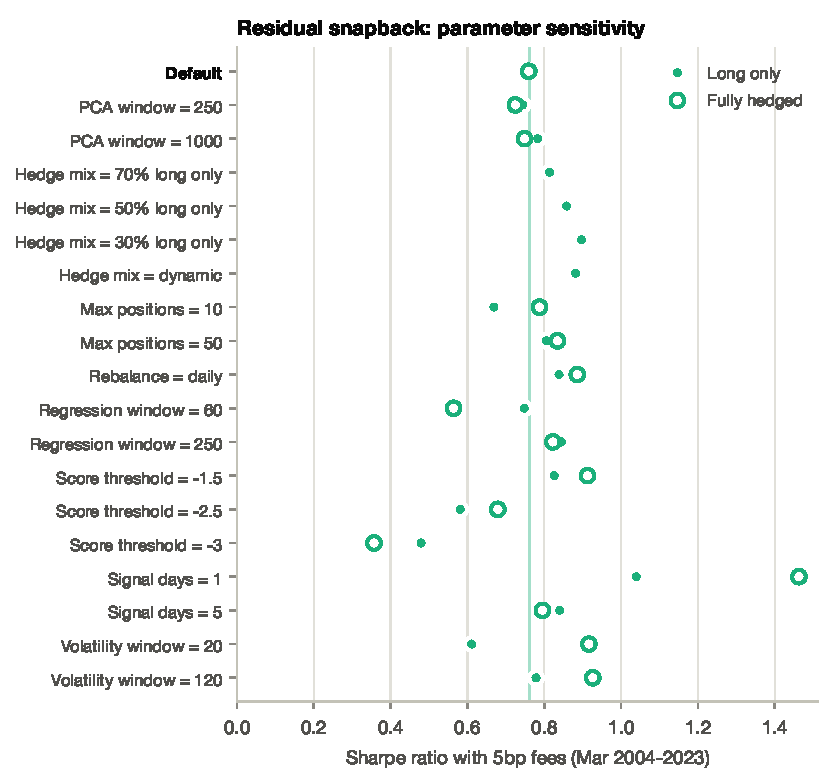
\includegraphics[width=0.7\textwidth]{figures/parameter_sensitivity_snap.pdf}
\caption{Sharpe ratio (5bp fees) of residual snapback for each parameter variant, long only (filled) and fully hedged (hollow). The vertical line marks the long-only default. Hedge mixes apply only to the long-only version.}
\label{fig:sensitivity-snap}
\end{figure}

\begin{figure}[H]
\centering
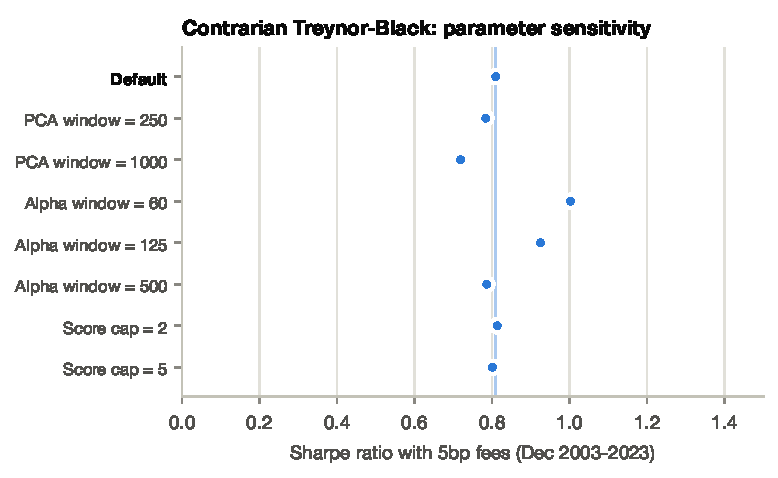
\includegraphics[width=0.7\textwidth]{figures/parameter_sensitivity_tb.pdf}
\caption{Sharpe ratio (5bp fees) of Contrarian Treynor--Black for each parameter variant. The vertical line marks the default settings.}
\label{fig:sensitivity-tb}
\end{figure}

\begin{figure}[H]
\centering
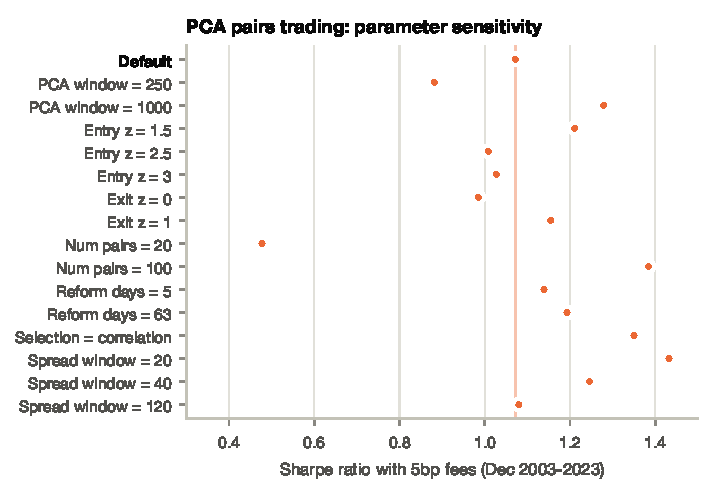
\includegraphics[width=0.7\textwidth]{figures/parameter_sensitivity_pairs.pdf}
\caption{Sharpe ratio (5bp fees) of PCA pairs trading for each parameter variant. The vertical line marks the default settings.}
\label{fig:sensitivity-pairs}
\end{figure}

\subsection{Trading costs}

\begin{table}[H]
\centering
\caption{Turnover and the cost of trading.}
\label{tab:costs}
\begin{tabular}{lcccc}
\toprule
& & & \multicolumn{2}{c}{Residual snapback} \\
\cmidrule(lr){4-5}
& Treynor--Black & Pairs trading & Long only & Fully hedged \\
\midrule
Daily turnover & 10.9\% & 5.6\% & 40.8\% & 40.3\% \\
Annual turnover & 28$\times$ & 14$\times$ & 103$\times$ & 102$\times$ \\
Gross return (annual mean) & 3.8\% & 3.6\% & 25.8\% & 11.3\% \\
Fee drag at 5bp (annual) & 1.4\% & 0.7\% & 5.2\% & 5.1\% \\
Share of edge lost at 5bp & 36\% & 20\% & 20\% & 45\% \\
Break-even fee & 14.0bp & 25.7bp & 25.0bp & 11.1bp \\
\midrule
Sharpe at 0bp & 1.31 & 1.45 & 1.03 & 1.38 \\
Sharpe at 2bp & 1.13 & 1.33 & 0.94 & 1.13 \\
Sharpe at 5bp & 0.85 & 1.17 & 0.82 & 0.76 \\
Sharpe at 10bp & 0.38 & 0.88 & 0.62 & 0.14 \\
Sharpe at 20bp & $-0.57$ & 0.32 & 0.21 & $-1.05$ \\
\bottomrule
\end{tabular}
\end{table}

Figures~\ref{fig:fees-tb}--\ref{fig:fees-snap} show how each strategy's Sharpe ratio falls with costs. Treynor--Black rebalances daily and turns over its portfolio 28 times a year, so costs take about a third of its edge, and it stops being profitable at around 14bp per trade. Pairs trading holds each position until the spread converges, halving turnover. It loses only a fifth of its edge to costs and survives fees up to about 26bp.

Residual snapback trades by far the most. Its holdings change almost completely every week, for a turnover of about 100 times a year, and fees cost 5\% a year at 5bp. The long-only version appears to survive this well (break-even 25bp), but only because its gross return includes the market, which costs nothing to trade. The fully hedged version, whose return is the strategy's own edge, loses 45\% of that edge at 5bp and breaks even at about 11bp, below Treynor--Black's 14bp. Trading costs are the main reason its Sharpe ratio of 1.38 before fees, close to pairs trading's 1.45, shrinks to 0.76.

\begin{figure}[H]
\centering
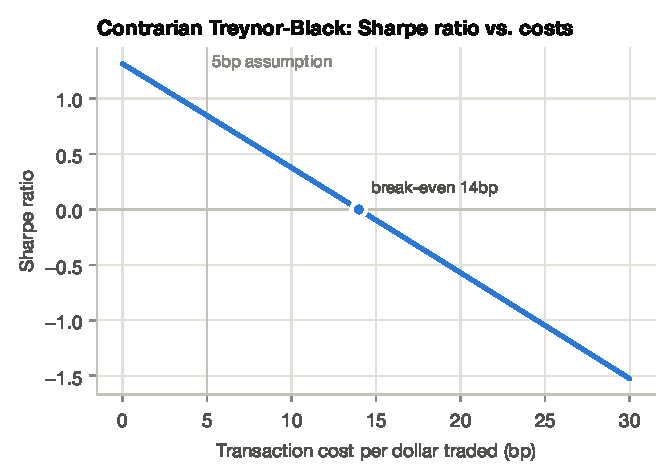
\includegraphics[width=0.65\textwidth]{figures/fee_sensitivity_tb.pdf}
\caption{Sharpe ratio of Contrarian Treynor--Black as a function of the transaction cost per dollar traded.}
\label{fig:fees-tb}
\end{figure}

\begin{figure}[H]
\centering
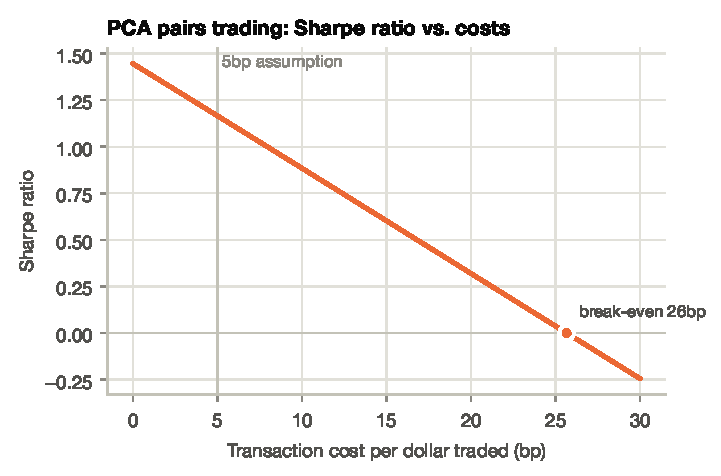
\includegraphics[width=0.65\textwidth]{figures/fee_sensitivity_pairs.pdf}
\caption{Sharpe ratio of PCA pairs trading as a function of the transaction cost per dollar traded.}
\label{fig:fees-pairs}
\end{figure}

\begin{figure}[H]
\centering
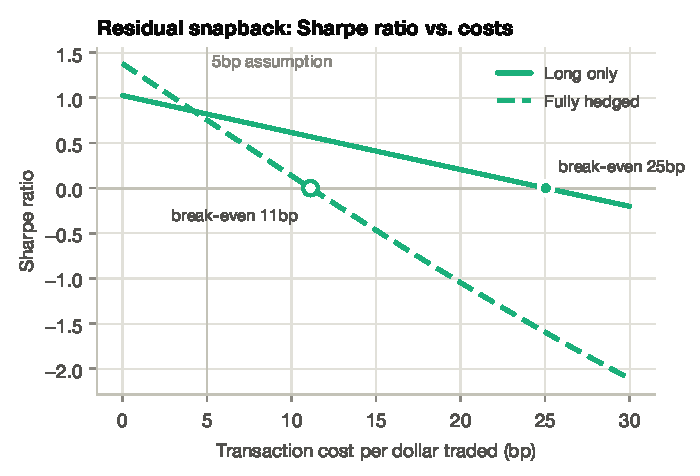
\includegraphics[width=0.65\textwidth]{figures/fee_sensitivity_snap.pdf}
\caption{Sharpe ratio of residual snapback, long only (solid) and fully hedged (dashed), as a function of the transaction cost per dollar traded.}
\label{fig:fees-snap}
\end{figure}

\subsection{Calibration}

To check that each signal predicts returns in the intended direction, we compare the signal on day $t$ with realized returns over the next $h$ days. For each day, we regress the realized return on the cross-sectionally standardized signal. Table~\ref{tab:calibration-slopes} reports the average slope with Newey--West $t$-statistics to account for overlapping horizons.

\begin{table}[H]
\centering
\caption{Treynor--Black: mean excess return by signal decile (bp).}
\label{tab:calibration-tb}
\begin{tabular}{lrrrrrrrrrr}
\toprule
Horizon & D1 & D2 & D3 & D4 & D5 & D6 & D7 & D8 & D9 & D10 \\
\midrule
1 day & $-3.0$ & $-2.0$ & $-1.3$ & $-1.0$ & 0.6 & 2.1 & 1.8 & 1.6 & 1.0 & 0.1 \\
5 days & $-10.7$ & $-6.6$ & $-1.7$ & $-1.0$ & 3.1 & 6.2 & 3.6 & 3.6 & 2.9 & 0.7 \\
20 days & $-34.4$ & $-17.4$ & $-0.5$ & 2.1 & 14.2 & 22.1 & 10.0 & 6.9 & 3.4 & $-6.1$ \\
\bottomrule
\end{tabular}
\\[4pt]
\small D1 is the decile the strategy shorts most (highest alpha), D10 the decile it buys most. Excess return is relative to the cross-sectional average.
\end{table}

\begin{table}[H]
\centering
\caption{Pairs trading: mean change in the pair's log price ratio by spread z-score (bp).}
\label{tab:calibration-pairs}
\begin{tabular}{lrrrr}
\toprule
Spread z-score & Next 1 day & Next 5 days & Next 20 days & Observations \\
\midrule
$z < -3$ & 48.4 & 108.4 & 157.9 & 2,251 \\
$-3$ to $-2$ & 17.7 & 20.8 & 43.9 & 16,811 \\
$-2$ to $-1$ & 7.0 & 13.5 & 8.3 & 56,696 \\
$-1$ to $0$ & 3.0 & 5.0 & $-0.8$ & 64,245 \\
$0$ to $1$ & $-3.5$ & $-6.3$ & $-31.8$ & 64,170 \\
$1$ to $2$ & $-7.2$ & $-14.3$ & $-53.1$ & 55,074 \\
$2$ to $3$ & $-18.3$ & $-46.2$ & $-101.7$ & 15,567 \\
$z > 3$ & $-59.7$ & $-143.8$ & $-267.5$ & 2,036 \\
\bottomrule
\end{tabular}
\end{table}

\begin{table}[H]
\centering
\caption{Residual snapback: mean excess return by snapback score (bp).}
\label{tab:calibration-snap}
\begin{tabular}{lrrrr}
\toprule
Snapback score $s_i$ & Next 1 day & Next 5 days & Next 20 days & Observations \\
\midrule
$s < -3$ & 13.1 & 46.6 & 67.1 & 52,973 \\
$-3$ to $-2$ & 10.8 & 25.8 & 40.4 & 118,870 \\
$-2$ to $-1$ & 9.7 & 17.4 & 24.5 & 653,346 \\
$-1$ to $0$ & 3.6 & 5.9 & 9.1 & 2,514,925 \\
$0$ to $1$ & $-4.2$ & $-6.8$ & $-9.5$ & 2,393,685 \\
$1$ to $2$ & $-7.7$ & $-15.2$ & $-27.0$ & 648,547 \\
$2$ to $3$ & $-9.3$ & $-22.9$ & $-34.4$ & 132,428 \\
$s > 3$ & $-18.3$ & $-42.8$ & $-39.4$ & 59,500 \\
\bottomrule
\end{tabular}
\\[4pt]
\small Every stock on every trading day, not only the stocks and weeks the strategy trades. Excess return is relative to the cross-sectional average. The strategy buys at $s \le -2$.
\end{table}

\begin{table}[H]
\centering
\caption{Cumulative residual score: mean excess return by score (bp).}
\label{tab:calibration-cumulative}
\begin{tabular}{lrrrr}
\toprule
Cumulative score $z_i$ & Next 1 day & Next 5 days & Next 20 days & Observations \\
\midrule
$z < -3$ & 19.8 & 60.5 & 86.3 & 83,025 \\
$-3$ to $-2$ & 8.8 & 18.7 & 32.2 & 408,691 \\
$-2$ to $-1$ & 3.9 & 8.5 & 17.8 & 1,282,369 \\
$-1$ to $0$ & 0.8 & 1.7 & 4.7 & 1,522,584 \\
$0$ to $1$ & $-0.7$ & $-2.2$ & $-3.6$ & 1,536,338 \\
$1$ to $2$ & $-4.2$ & $-8.9$ & $-19.7$ & 1,262,177 \\
$2$ to $3$ & $-8.5$ & $-19.6$ & $-38.0$ & 397,668 \\
$z > 3$ & $-19.4$ & $-45.7$ & $-56.9$ & 83,824 \\
\bottomrule
\end{tabular}
\\[4pt]
\small Same stocks, days and target as Table~\ref{tab:calibration-snap}, using the lagged factor model's residuals. Observations are for the next-day horizon.
\end{table}

\begin{table}[H]
\centering
\caption{Return per one standard deviation of signal.}
\label{tab:calibration-slopes}
\resizebox{\textwidth}{!}{%
\begin{tabular}{lrrrrrrrr}
\toprule
& \multicolumn{2}{c}{Treynor--Black} & \multicolumn{2}{c}{Pairs trading} & \multicolumn{2}{c}{Snapback score} & \multicolumn{2}{c}{Cumulative score} \\
\cmidrule(lr){2-3} \cmidrule(lr){4-5} \cmidrule(lr){6-7} \cmidrule(lr){8-9}
Horizon & Slope & $t$-stat & Slope & $t$-stat & Slope & $t$-stat & Slope & $t$-stat \\
\midrule
1 day & 1.1bp & 5.2 & 9.6bp & 13.3 & 6.0bp & 21.6 & 5.0bp & 18.1 \\
5 days & 3.4bp & 3.4 & 19.3bp & 7.3 & 11.4bp & 13.3 & 11.1bp & 10.9 \\
20 days & 7.7bp & 1.8 & 39.0bp & 4.7 & 17.1bp & 10.7 & 20.6bp & 7.4 \\
\bottomrule
\end{tabular}}
\\[4pt]
\small The pairs slope is per pair spread; the Treynor--Black and snapback slopes are per stock.
\end{table}

The pairs signal is very well calibrated (Figures~\ref{fig:calibration-tb} and~\ref{fig:calibration-pairs}). Future spread returns fall steadily with the z-score in every bucket and at every horizon, and the relationship is highly significant ($t = 13.3$ at one day). The Treynor--Black signal is significant at short horizons ($t = 5.2$) but only partly monotonic. Its predictive power is concentrated in the stocks it shorts: the highest-alpha decile underperforms strongly and persistently. The lowest-alpha stocks it buys most do not outperform, and at 20 days they underperform. In other words, high past alpha reverses, but very low past alpha does not. The edge also fades with horizon, consistent with the strategy's need for daily rebalancing.

The snapback score is as well calibrated as the pairs signal and the most statistically significant of the three (Figure~\ref{fig:calibration-snap}). Future excess returns fall monotonically across all eight score buckets at every horizon, and the slope has the highest $t$-statistic of any signal (21.6 at one day, still 10.7 at 20 days), helped by the much larger number of observations. Stocks in the buy zone ($s \le -2$) beat the cross-section by 26--47bp over the following week. The relationship is symmetric: stocks with unusually \emph{positive} residuals underperform just as reliably, which is what the fully hedged version's short leg exploits. Because the signal is so well calibrated, the strategy's modest Sharpe ratio comes from how the signal is traded (the market exposure of the long-only version and the heavy turnover), not from the signal itself.

The cumulative score is also monotonic in every bucket at every horizon (Table~\ref{tab:calibration-cumulative}). Its slope is slightly smaller than the snapback score's at one day (5.0bp vs.\ 6.0bp) but larger at 20 days (20.6bp vs.\ 17.1bp), and its most extreme buckets have larger returns ($+60$bp over five days for $z < -3$, against $+47$bp for the snapback score). This fits the execution-delay results: the cumulative score's predictive power lasts longer, so less of it is lost when trading weekly or a day late.

\begin{figure}[H]
\centering
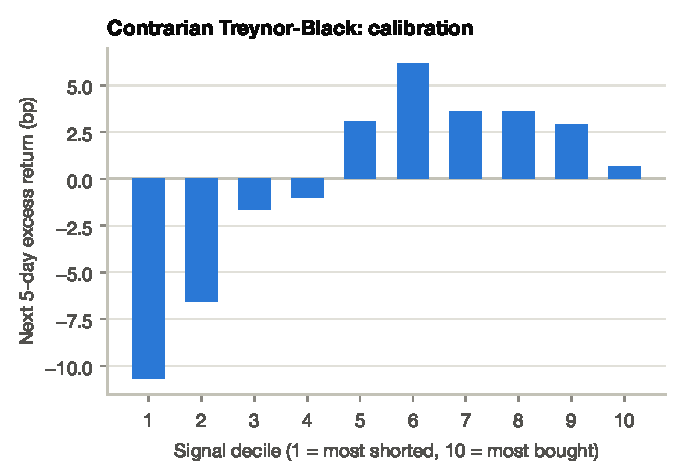
\includegraphics[width=0.65\textwidth]{figures/calibration_tb.pdf}
\caption{Calibration of Contrarian Treynor--Black: next 5-day excess return by signal decile.}
\label{fig:calibration-tb}
\end{figure}

\begin{figure}[H]
\centering
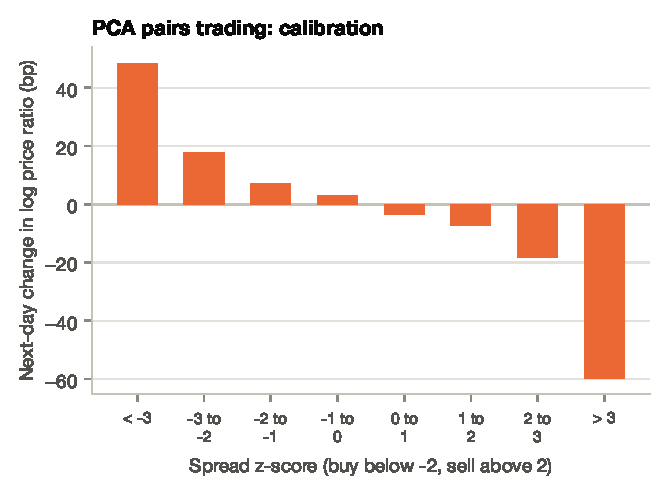
\includegraphics[width=0.65\textwidth]{figures/calibration_pairs.pdf}
\caption{Calibration of PCA pairs trading: next-day change in the pair log price ratio by spread z-score.}
\label{fig:calibration-pairs}
\end{figure}

\begin{figure}[H]
\centering
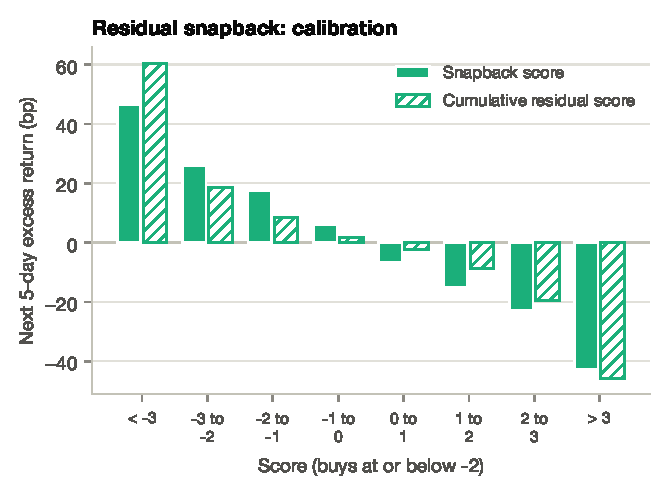
\includegraphics[width=0.65\textwidth]{figures/calibration_snap.pdf}
\caption{Calibration of residual snapback (Tables~\ref{tab:calibration-snap} and~\ref{tab:calibration-cumulative}): next 5-day excess return by snapback score (solid) and by cumulative residual score (hatched).}
\label{fig:calibration-snap}
\end{figure}

\begin{figure}[H]
\centering
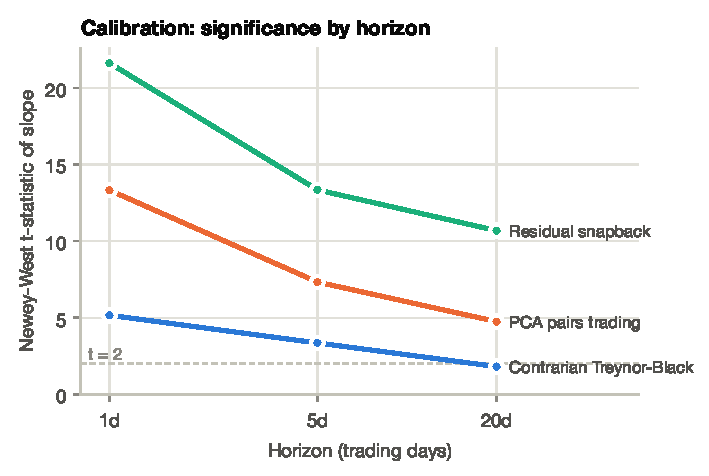
\includegraphics[width=0.65\textwidth]{figures/calibration_slopes.pdf}
\caption{Newey--West $t$-statistic of each signal's slope by horizon (Table~\ref{tab:calibration-slopes}); the cumulative residual score is dashed. The gray dashed line marks $t = 2$. The $t$-statistics are comparable across strategies even though the slopes are in different units.}
\label{fig:calibration-slopes}
\end{figure}

\subsection{Holdout}
\label{sec:holdout}

To check that our design choices are not overfit, we treat 2018--2023 as a holdout. Any choice is made using only 2002--2017 data and then evaluated once on the holdout.

\begin{table}[H]
\centering
\caption{Selection period vs.\ holdout (Sharpe ratios, 5bp fees).}
\label{tab:holdout}
\begin{tabular}{llrr}
\toprule
Strategy & Choice & 2002--2017 & 2018--2023 \\
\midrule
Treynor--Black & Default settings & 1.08 & 0.40 \\
& Best setting on 2002--2017 (alpha window 60) & 1.13 & 0.83 \\
& Best $K$ on 2002--2017 ($K = 20$) & 1.11 & 0.63 \\
Pairs trading & Default settings & 1.04 & 1.15 \\
& Best setting on 2002--2017 (spread window 20) & 1.63 & 1.05 \\
& Best $K$ on 2002--2017 ($K = 15$) & 1.41 & 0.58 \\
Snapback, long only & Default settings & 0.83 & 0.62 \\
& Best setting on 2002--2017 (1 signal day) & 1.23 & 0.69 \\
& Best $K$ on 2002--2017 ($K = 5$, the default) & 0.91 & 0.62 \\
& Best hedge mix on 2002--2017 (dynamic) & 1.06 & 0.51 \\
Snapback, fully hedged & Default settings & 0.87 & 0.59 \\
& Best setting on 2002--2017 (1 signal day) & 1.71 & 1.03 \\
& Best $K$ on 2002--2017 ($K = 3$) & 0.98 & 0.79 \\
\midrule
Following alpha (no fees) & Sign check & $-1.63$ & $-0.77$ \\
\bottomrule
\end{tabular}
\\[4pt]
\small Default, best-setting and hedge-mix rows use the common period of the parameter variants, starting December 2003 (March 2004 for snapback). Best-$K$ rows start in 2002, so the $K = 5$ row differs slightly from the default row.
\end{table}

\begin{figure}[H]
\centering
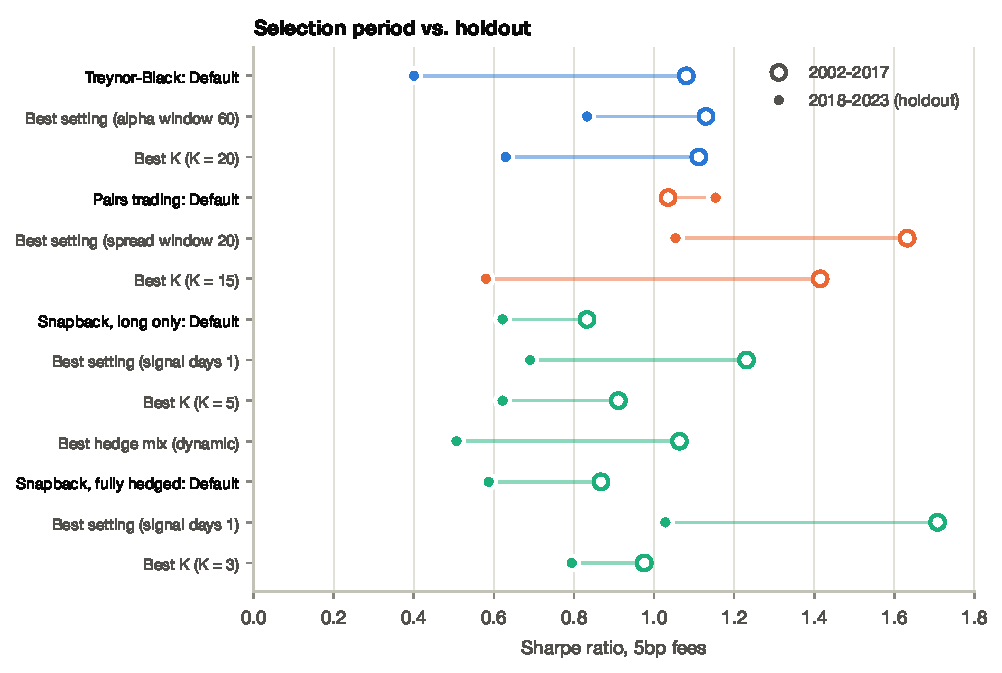
\includegraphics[width=0.85\textwidth]{figures/holdout.pdf}
\caption{Selection period vs.\ holdout (Table~\ref{tab:holdout}): Sharpe ratio with 5bp fees in 2002--2017 (hollow) and in the 2018--2023 holdout (filled). The no-fee sign check is omitted.}
\label{fig:holdout}
\end{figure}

Four results stand out. First, the contrarian direction is justified using the selection period alone: following alpha loses money in 2002--2017 (Sharpe $-1.63$), so reversing the sign was not chosen by looking at the full sample. Second, pairs trading holds up in the holdout (Sharpe 1.15, versus 1.04 before). Optimizing its parameters on the selection period did \emph{not} help: every optimized choice did worse in the holdout than the defaults, the classic signature of overfitting. Third, Treynor--Black weakens substantially in the holdout (Sharpe 0.40 with default settings), consistent with the decline in its second-half performance in Table~\ref{tab:regime}.

Fourth, residual snapback weakens in the holdout but less than Treynor--Black (0.62 long only and 0.59 hedged, from 0.83 and 0.87). Unlike for the other two strategies, some choices made on the selection period carried over. The one-day signal beat the default in the holdout in both versions (0.69 vs.\ 0.62 long only, 1.03 vs.\ 0.59 hedged), and $K = 3$ helped the hedged version (0.79). The best hedge mix on 2002--2017, the dynamic volatility mix, did not: it reached only 0.51 in the holdout, below the long-only default. Even where choices carried over, the holdout gains were smaller than the selection-period gains (for the one-day signal, $+0.07$ vs.\ $+0.40$ long only and $+0.44$ vs.\ $+0.84$ hedged), so part of the apparent improvement is overfitting.

\subsection{Number of factors $K$}

Finally, we re-run all three strategies for $K \in \{1, 2, 3, 5, 8, 10, 15, 20\}$, both out-of-sample and in-sample. In the in-sample version, the PCA and the alphas are estimated once on the full 2000--2023 sample and then traded over the same period, which introduces look-ahead bias. For residual snapback, the in-sample version computes each day's residual from the full-sample coefficients.

\begin{table}[H]
\centering
\caption{Sharpe ratios by number of factors $K$.}
\label{tab:k}
\begin{tabular}{rrrrrrrr}
\toprule
& \multicolumn{4}{c}{Treynor--Black} & \multicolumn{3}{c}{Pairs trading} \\
\cmidrule(lr){2-5} \cmidrule(lr){6-8}
& \multicolumn{2}{c}{Out-of-sample} & \multicolumn{2}{c}{In-sample} & \multicolumn{2}{c}{Out-of-sample} & In-sample \\
\cmidrule(lr){2-3} \cmidrule(lr){4-5} \cmidrule(lr){6-7}
$K$ & No fees & 5bp & Contrarian & Follow $\alpha$ & No fees & 5bp & No fees \\
\midrule
1 & 0.95 & 0.68 & $-1.54$ & 1.54 & 0.78 & 0.52 & 0.62 \\
2 & 0.86 & 0.54 & $-2.12$ & 2.12 & 1.39 & 1.11 & 0.69 \\
3 & 0.87 & 0.51 & $-2.13$ & 2.13 & 1.13 & 0.86 & 1.13 \\
5 & 1.31 & 0.85 & $-2.18$ & 2.18 & 1.45 & 1.17 & 1.93 \\
8 & 1.46 & 0.92 & $-2.76$ & 2.76 & 1.41 & 1.09 & 2.18 \\
10 & 1.49 & 0.91 & $-2.77$ & 2.77 & 1.53 & 1.18 & 2.40 \\
15 & 1.58 & 0.94 & $-3.29$ & 3.29 & 1.51 & 1.14 & 2.39 \\
20 & 1.66 & 0.96 & $-3.42$ & 3.42 & 1.60 & 1.18 & 2.15 \\
\bottomrule
\end{tabular}
\end{table}

\begin{figure}[H]
\centering
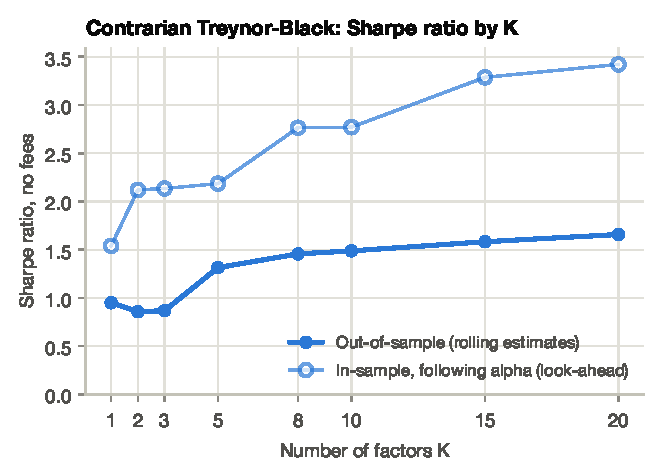
\includegraphics[width=0.65\textwidth]{figures/k_sweep_tb.pdf}
\caption{Sharpe ratio (no fees) of Contrarian Treynor--Black by number of factors $K$, out-of-sample vs.\ in-sample. The in-sample version follows alpha rather than trading against it.}
\label{fig:k-tb}
\end{figure}

\begin{figure}[H]
\centering
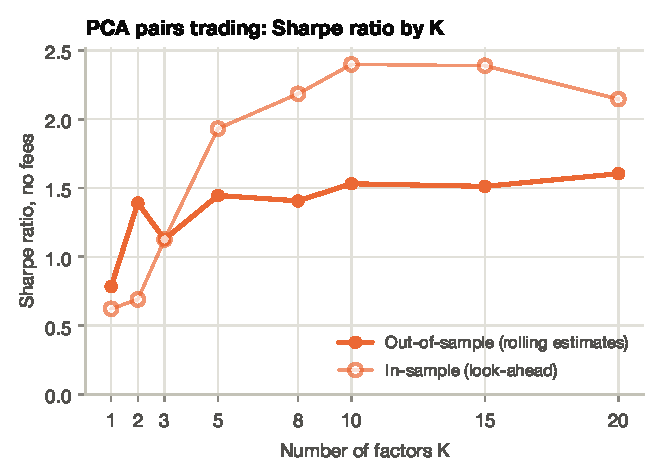
\includegraphics[width=0.65\textwidth]{figures/k_sweep_pairs.pdf}
\caption{Sharpe ratio (no fees) of PCA pairs trading by number of factors $K$, out-of-sample vs.\ in-sample.}
\label{fig:k-pairs}
\end{figure}

\begin{table}[H]
\centering
\caption{Sharpe ratios by number of factors $K$: residual snapback.}
\label{tab:k-snap}
\begin{tabular}{rrrrrrr}
\toprule
& \multicolumn{3}{c}{Long only} & \multicolumn{3}{c}{Fully hedged} \\
\cmidrule(lr){2-4} \cmidrule(lr){5-7}
& \multicolumn{2}{c}{Out-of-sample} & In-sample & \multicolumn{2}{c}{Out-of-sample} & In-sample \\
\cmidrule(lr){2-3} \cmidrule(lr){5-6}
$K$ & No fees & 5bp & No fees & No fees & 5bp & No fees \\
\midrule
1 & 1.01 & 0.81 & 1.03 & 1.41 & 0.89 & 1.40 \\
2 & 1.02 & 0.82 & 1.01 & 1.31 & 0.78 & 1.52 \\
3 & 1.03 & 0.82 & 1.07 & 1.53 & 0.91 & 1.64 \\
5 & 1.03 & 0.82 & 1.18 & 1.38 & 0.76 & 1.84 \\
8 & 1.00 & 0.79 & 1.13 & 1.50 & 0.77 & 1.86 \\
10 & 0.98 & 0.77 & 1.16 & 1.38 & 0.65 & 1.93 \\
15 & 1.01 & 0.80 & 1.12 & 1.01 & 0.29 & 1.88 \\
20 & 0.98 & 0.77 & 1.12 & 0.46 & $-0.21$ & 1.97 \\
\bottomrule
\end{tabular}
\end{table}

\begin{figure}[H]
\centering
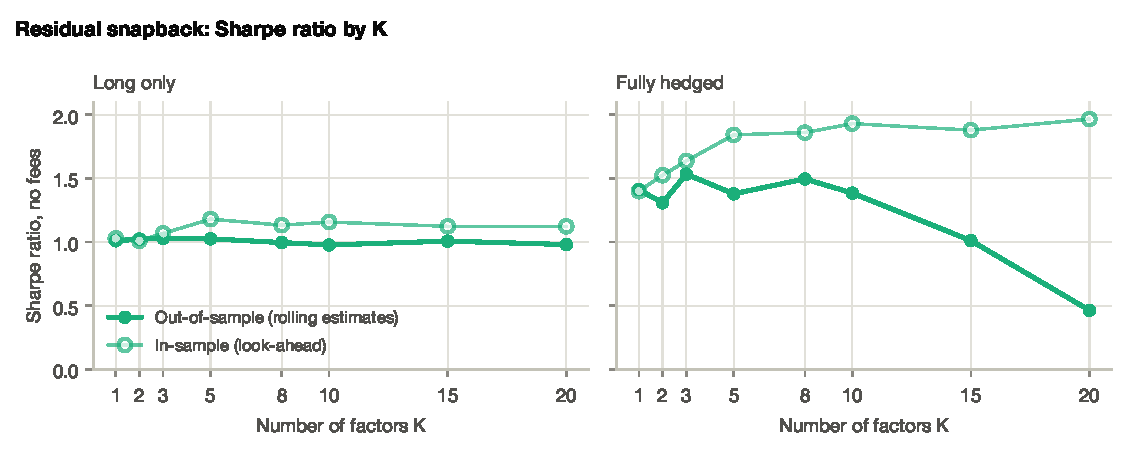
\includegraphics[width=0.65\textwidth]{figures/k_sweep_snap.pdf}
\caption{Sharpe ratio (no fees) of residual snapback by number of factors $K$, out-of-sample vs.\ in-sample, long only (left) and fully hedged (right).}
\label{fig:k-snap}
\end{figure}

\paragraph{In-sample vs.\ out-of-sample.} The difference is dramatic (Figures~\ref{fig:k-tb} and~\ref{fig:k-pairs}). In-sample, following alpha appears highly profitable, with Sharpe ratios of 2 to 3.4 that rise as more factors are added. This is look-ahead bias: the full-sample alpha is estimated from the very returns being traded, so stocks with high alpha mechanically earned high returns over the period. Out-of-sample, the same signal points the \emph{opposite} way: high past alpha predicts low future returns. An in-sample assessment would not just overstate performance; it would recommend the wrong strategy. Pairs trading is also inflated in-sample (Sharpe up to 2.4 vs.\ about 1.5 out-of-sample), though its direction is unchanged. Long-only residual snapback is the least affected (Figure~\ref{fig:k-snap}): its in-sample Sharpe ratios exceed out-of-sample ones by at most 0.18. Its signal is a short-lived residual relative to a stock's own recent volatility, which full-sample coefficients barely change, rather than an estimate of the long-run alpha that look-ahead contaminates directly. The hedged version is affected much more, increasingly so as $K$ grows (1.84 vs.\ 1.38 at $K = 5$, 1.97 vs.\ 0.46 at $K = 20$). Its hedge relies on the betas, and full-sample betas describe the factor exposures over the very period being traded, so in-sample the hedge removes factor risk almost perfectly. Out-of-sample, each extra factor adds another set of estimated betas to hedge against, and their estimation error accumulates.

\paragraph{Which $K$ works best?} Out-of-sample, performance improves up to roughly $K = 5$--$8$ and then levels off, especially after fees. For Treynor--Black, the Sharpe ratio after fees is 0.85 at $K = 5$ and only 0.96 at $K = 20$. For pairs trading, every $K \ge 2$ gives a Sharpe ratio between 0.86 and 1.18 after fees. Picking $K$ by its past performance also did not carry over to the holdout for Treynor--Black or pairs trading (Table~\ref{tab:holdout}). Long-only snapback is insensitive to $K$ (0.77--0.82 after fees for every value). The hedged version prefers \emph{few} factors: after fees it does best at $K = 1$--$3$ (0.78--0.91) and deteriorates beyond $K = 8$ (0.29 at $K = 15$, $-0.21$ at $K = 20$), because each extra factor to neutralize forces the weights further from the signal and adds estimation noise to the hedge. We therefore keep $K = 5$ for all three strategies: it captures most of the benefit, and larger values add estimation noise without a reliable improvement.

\section{Conclusion}

All three PCA strategies are profitable out-of-sample and after transaction costs, but they differ in robustness. Contrarian Treynor--Black shows that estimated alphas reverse rather than persist. It is factor neutral by construction (market beta 0.04) and performs best in crises, but it is concentrated in 2008--09, sensitive to trading costs, and has weakened since 2013. PCA pairs trading is the most robust strategy: it is profitable in 21 of 22 years, well calibrated, insensitive to its parameters, and stronger in the 2018--2023 holdout than before it. Residual snapback has the strongest signal of the three, with stocks that fall well short of the factor model's prediction reliably outperforming over the next one to twenty days. Its implementation leaves much of that signal on the table. The long-only version mostly earns the market return (beta 1.08, the same Sharpe ratio as an equal-weight benchmark), and the fully hedged long-short version, comparable to the other two strategies, has a Sharpe ratio of 1.38 before fees but trades about 100 times a year and gives up almost half of its edge to costs. Both weaken in the holdout, and the hedged version's edge has faded since 2013. Measuring the shortfall cumulatively rather than over three days helps most: with the same trading rules, the cumulative residual score raises the long-short Sharpe ratio after fees to 1.76 (1.26 in the holdout) and keeps 1.07 when trades are executed a day late. A daily version of the same signal reaches 3.01, but it collapses to 0.25 with a one-day delay. Most of its profit comes from next-day price reversals that a real trader could probably not capture. Finally, the contrast between in-sample and out-of-sample results shows why rolling estimation matters. Estimating the model on the full sample does not merely inflate performance; for Treynor--Black it reverses the conclusion about which way to trade.

\end{document}
